\section{Architecture and rationale of EPS}
\label{sec:EPS_architecture_rationale}

\subsection{Available alternatives}
\label{subsec:available_alternatives}

The endeavour that Juno faces to generate enough electricity to sustain science operations at 5.44 AU required particular attention in designing an efficient and reliable electric control system. Particularly, different options were present to generate the amount of power required, each of them with advantages and disadvantages:

\begin{itemize}
    \item \textbf{RTG:} the choice of a radioisotope to generate electricity could be considered. In order to generate the amount of power required around Jupiter, during the planetary phase 
    (\mref), 
    one RTG of the same size of the one present on board New Horizons spacecraft  would have been sufficient ( $\approx$ 250 We of production at BOL)\cite{nh_rtg}. Electric power requirement would also be lower as some heat could have been routed to the propulsion section to heat up the tanks and fuel lines. This choice however had some problems, mainly with respect to the safety during Earth EGA, radiation contamination, heat dissipation at distances lower than 2 AU from the Sun and weight distribution. Particular problems could have rose as the said RTG generates around 4.4 kW of heat, requiring a very efficient dissipation system for the first years of the mission, oversizing it with respect to the nominal orbit around Jupiter. Availability of Plutonium-238 was also critical as suppliers could not guarantee the needed amount of fuel, given the stop in the production of the said isotope during the 80s. 
    \mref % ---- eventualmente da approfondire ----- 
    \item \textbf{Solar panels:} no spacecraft equipped with solar panels has ever been tested at 5.44 AU from the Sun. This choice would have required a very large surface area, and thus precautions had to be taken into account inside the fairing during launch operations, to provide enough power for safe operations at Jupiter. A complex management system is also required in order to not discharge too much current inside the electronics during the ICs and the OC as the amount of solar flux hitting the S/C during different parts of the mission dramatically reduces. More stringent pointing requirements are also present as not having a clear view of the Sun could have led to the need of bigger and heavier batteries. 
\end{itemize}

Considering also the driving requirement of utilizing as much as possible off the shelf components, budget constraints, the limited supply of plutonium and the different possible configurations offered, solar panels were chosen. This choice led to a particular design of the satellite, where mass distribution was exploited to grant more stability throughout the different phases of the mission.  

\subsection{Components and distribution}
\label{subsec:components_and_distribution}

The flown spacecraft is fitted with 3 solar arrays and 2 Li-On batteries. 

\begin{itemize}

\item The arrays are mounted on the side of the main body, spaced 120° apart, and are composed by a different number of panels, as can be seen in \autoref{table:panels_area}: solar wing 1 presents only 3 panels while solar wing 2 and 3 present 4 panels each. Solar panels are linked one to the other and to the main body with electro-actuated hinges and the first panel of each array is supported by struts. All these elements are needed to both extend the panels soon after separation from the Centaur and to control the position of the arrays during all the operations. This is necessary to take into account the bending of the arrays during large manuevers and their thermal expansion. Moreover it is necessary to align the main inertia axis (Z-axis) with the spin axis as the three solar arrays do not feature an exactly symmetrical mass distribution due to the presence of the MAG boom.
However, using different dimensions for each set of panels allowed to minimize the effect of the said asymmetry. From \autoref{table:panels_area} the area of each panel can be observed: A2 and A3 feature identical panels distribution while A1 presents only 3 panels. Once the power requirement is fixed, each panels area was defined to optimize the inertia matrix.   




Each panel is composed by gnagna

This  difference is due to the presence of the MAG boom. As a large area to be irradiated is crucial, solar arrays extend 

\end{itemize}
% disposizione pannelli: dimensioni, posizionamento, ripercussioni sulla dinamica. riferimenti tab e figure

% --- l'immagine è ancora da fare, è per avere idea delle dimensioni ---
\begin{minipage}{0.5\linewidth}
    \centering
    \captionsetup{type=figure}
    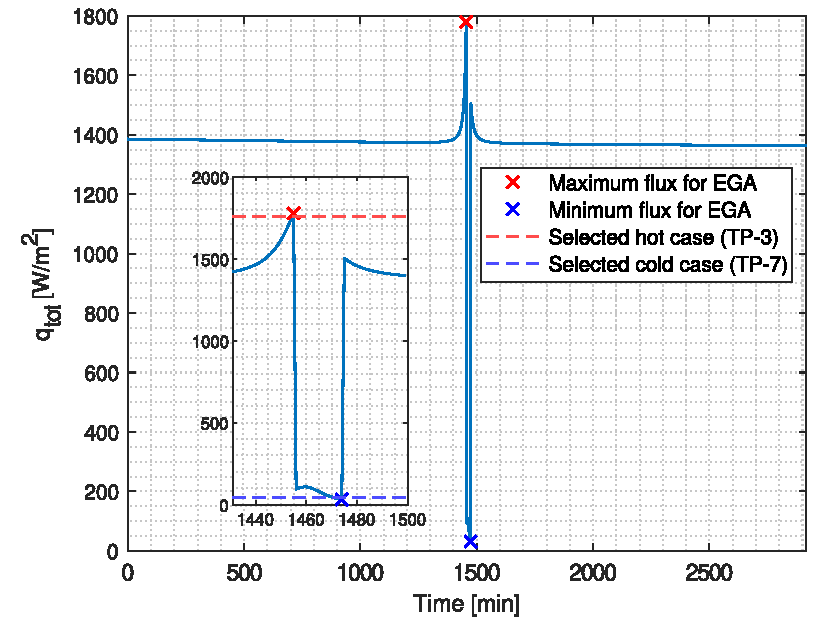
\includegraphics[width=\linewidth]{Images/EGA_flux_analysis.pdf}
    \caption{Juno's panel configuration}
    \label{fig:panel_config}
\end{minipage}\hfill
\begin{minipage}{0.5\linewidth}
    \centering
    \captionsetup{type=table}
    \renewcommand{\arraystretch}{1.4}
    \begin{tabular}{|c|c|c|c|c|}
        \hline
        &  \textbf{P1}  & \textbf{P2} & \textbf{P3} & \textbf{P4}\\
        \hline
        \hline
        \textbf{A1}      & 4.92 & 5.60 & 5.60 & - \\
        \hline
        \textbf{A2}      & 4.81 & 5.46 & 5.46 & 6.29  \\
        \hline
        \textbf{A3}     & 4.81 & 5.46 & 5.46 & 6.29  \\
        \hline
    \end{tabular}
    \caption{Panels areas [m$^2$]}
    \label{table:panels_area}
\end{minipage}

% struttura pannelli, numero celle, divisione stringhe, funzionamento delle stringhe 

% ------ come varia la distanza dal sole, angolo 

